\chapter{State of the art}
\label{chapter2}

Over the last few years, the main idea of this project has been broadly discussed and developed by other researchers. As such, there has been several projects that aimed to provide ingredient scanning tools for allergy patients on the literature. However, the popularity of user-ready applications that successfully implement this concept is reduced, as the few apps that have had a surge in popularity do not work nearly as well when dealing with food allergies. There are, however, some niche applications that effectively manage to implement a solution suited for patients of food intolerance.

In this chapter, we will select and discuss some of this projects, both from academic sources as well as commercial solutions freely available on app store platforms, in order to build a general picture about some of the recent developments made on this field.

\section{Literature review}

The central concept for this mobile application idea, text recognition over an ingredients list, has already been explored to some extent by previous authors, using different approaches which will serve as the foundation for the development of the application. On the following section two recent papers (from 2020 and 2021) that addressed the same problem will be discussed. The goal is to draw a comparison and highlight the differences between their proposed solution and the one intended for development during this project.

\subsection{Kamis and Shin}

Kamis and Shin \cite{putri_kamis_ocr-based_2020} used a similar approach to the intended in this project, performing OCR over the ingredients list in the package and refining this result using NLP techniques. Despite the recency of this paper, it provides a very robust framework in its solution that may be suited for all sort of similar applications. An adaptation of the implementation proposed in this paper, which also served as an initial guideline for this project, is shown in Figure \ref{fig:kamis}.

\begin{figure}[h]
  \centering
  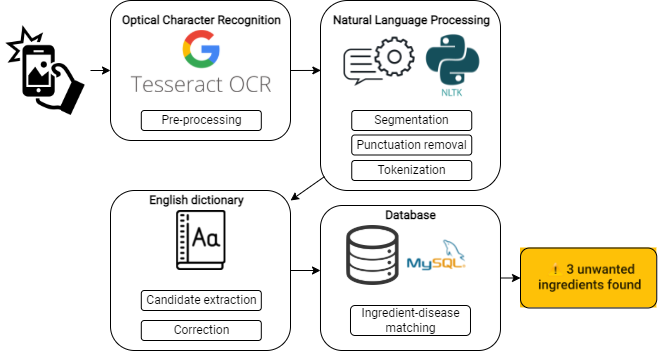
\includegraphics[width=\textwidth]{Figures/kamis.png}
  \caption{%
    Implementation schema proposed by Kamis and Shin
  }
  \label{fig:kamis}
\end{figure}

The one main difference is that this paper is designed entirely to work with English language and Latin script. Our project aims, however, to be used on Korean sources, which limits the range and effectiveness of OCR solutions available. \textit{Hangeul} text recognition is less trivial and systems are usually less refined and accurate for this script, which heavily deviates from the ubiquitous Latin script. In the same way, the array of data sources and processing tools is also more limited when working with Korean language, so other solutions will need to be found. Finally, the language barrier between the user and the input will also need to be addressed using a predefined database as well as an automated translation service.

\subsection{Jacky and Ma'muriyah}

Jacky and Ma'muriyah \cite{mamuriyah_perancangan_2021} have also developed a variation of this project, where the input taken is just the name of the food or dish and the ingredients are retrieved from a database. Other works from Korean authors \cite{lee_development_2017,yoon_web-app_2021} have taken the same approach to solving the problem. In this paper the developed application works over both \textit{hangeul} food names as well as romanized ones, although the accuracy achieved is higher when working with the latter. In Figure \ref{fig:kamis} we can see a practical example of their application correctly reading the name of a traditional Korean dish.

\begin{figure}[h]
  \centering
  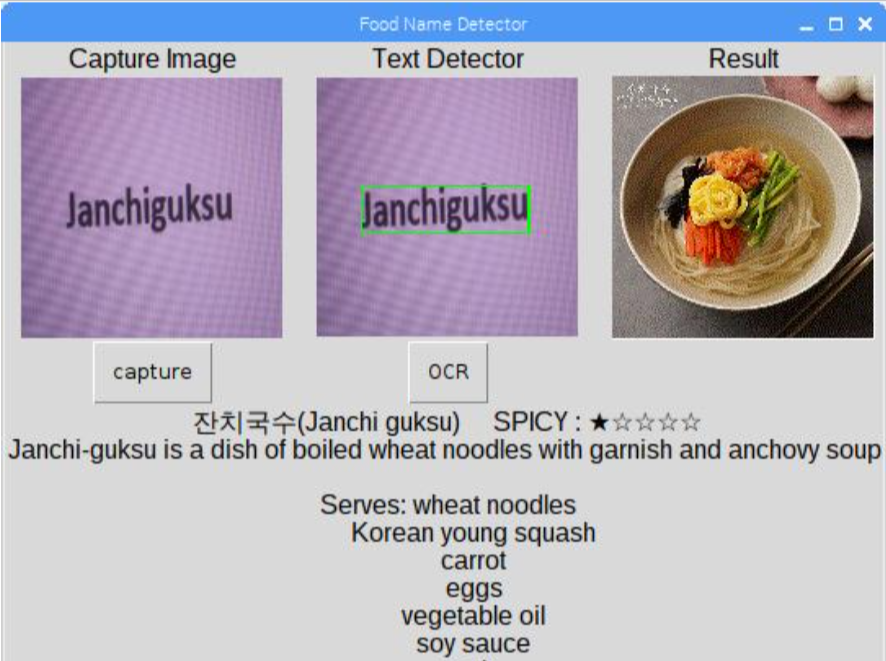
\includegraphics[width=0.5\textwidth]{Figures/jacky.png}
  \caption{%
    Execution example of the app developed by Jacky and Ma'muriyah
  }
  \label{fig:jacky}
\end{figure}

The main difference is that the project defined in this DFP aims to directly retrieve the ingredient list independent of the specific name of the product, so as to eliminate the need of maintaining an ever-changing database. This ensures that the application should work even on the newest of food products, as long as the ingredient list is humanly readable.

\section{Similar applications}

On this section, we will discuss some applications based on ideas that are similar to the subject of this project, detail its main features and compare them to the ones that our application implements.

\subsection{Yuka}

It should be noted that \textit{Yuka} \cite{noauthor_yuka_nodate-1} is not advertised as a food allergy-oriented ingredient scanner, and is more of a quality index provider for food products based on their added additives and nutritional information. However, given its huge popularity with more than 10 million downloads and 75.000 ratings \cite{noauthor_yuka_nodate} (which represents figures a thousand times higher than other apps in this section), it is included in this compilation. Its logotype is shown in Figure \ref{fig:yuka}.

\begin{figure}[h]
  \centering
  
\includegraphics[width=0.5\textwidth]{Figures/yuka.png}
  \caption{%
    Yuka's logotype
  }
  \label{fig:yuka}
\end{figure}

Despite not being specifically a scanner for food intolerances, it is capable of presenting the ingredients list for some of the items on their databases, and even supports new additions by taking a picture of the ingredients list. However, their OCR system does not support Korean language, therefore it is currently impossible to register products with packaging in Korean or attempt to scan their ingredients. For the products where it does work, there is no option present to set an alert in case a determinate ingredient is found, so the user should read and scan through the list manually. Some screenshots of the app interface can be seen on Figure \ref{fig:yuka-screenshot}.

\begin{figure}[h]
    \centering
    \begin{subfigure}{0.3\textwidth}
        \centering
        \includegraphics[width=0.9\linewidth]{Figures/Yuka-1.jpg}
        \caption{}
        \label{fig:yuka-1}
    \end{subfigure}
    \begin{subfigure}{0.3\textwidth}
        \centering
        \includegraphics[width=0.9\linewidth]{Figures/Yuka-2.jpg}
        \caption{}
        \label{fig:yuka-2}
    \end{subfigure}
    \begin{subfigure}{0.3\textwidth}
        \centering
        \includegraphics[width=0.9\linewidth]{Figures/Yuka-3.jpg}
        \caption{}
        \label{fig:yuka-3}
    \end{subfigure}
    \caption{Yuka app screenshots}
    \label{fig:yuka-screenshot}
\end{figure}

It supports barcode scanning as the main method for recognizing a product, with a prompt for OCR scanning if it has not been registered in their database yet. Because of this, the app will logically not function if the device is not connected to the Internet. On the UI aspect, \textit{Yuka} has a very clean and simple interface which will serve as inspiration for our mobile application.

\subsection{Soosee}

\textit{Soosee} \cite{noauthor_soosee_nodate-1} is a food scanner app specially developed for people with food allergies or intolerances. Its interface and functioning is quite simplified, with only three differentiated screens. On the secondary screen you can toggle which ingredients you want to detect, while on the main screen the detected allergens will appear highlighted on real time. Its logotype is shown in Figure \ref{fig:soosee}.

\begin{figure}[h]
  \centering
  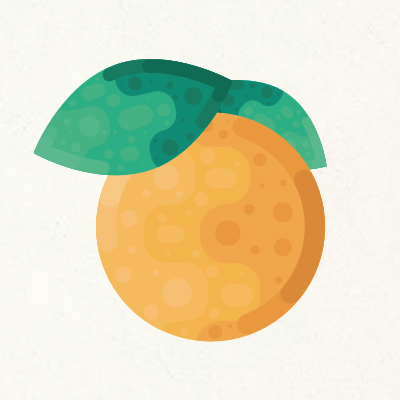
\includegraphics[width=0.25\textwidth]{Figures/soosee.png}
  \caption{%
    Soosee's logotype
  }
  \label{fig:soosee}
\end{figure}

Although this app is nearly not as popular as \textit{Yuka}, with around 10.000 total installs \cite{noauthor_soosee_nodate}, it is much more similar in its way of functioning to our target app. The main differences are that \textit{Soosee} does not support Korean language and that it does not support adding new ingredients, having only the option to toggle the existing ones. On the other hand, it features real-time scanning, which is a feature left out of the scope of our app. The main screens of \textit{Soosee} are shown on the screenshots in Figure \ref{fig:soosee-screenshot}.

\begin{figure}[h]
    \centering
    \begin{subfigure}{0.3\textwidth}
        \centering
        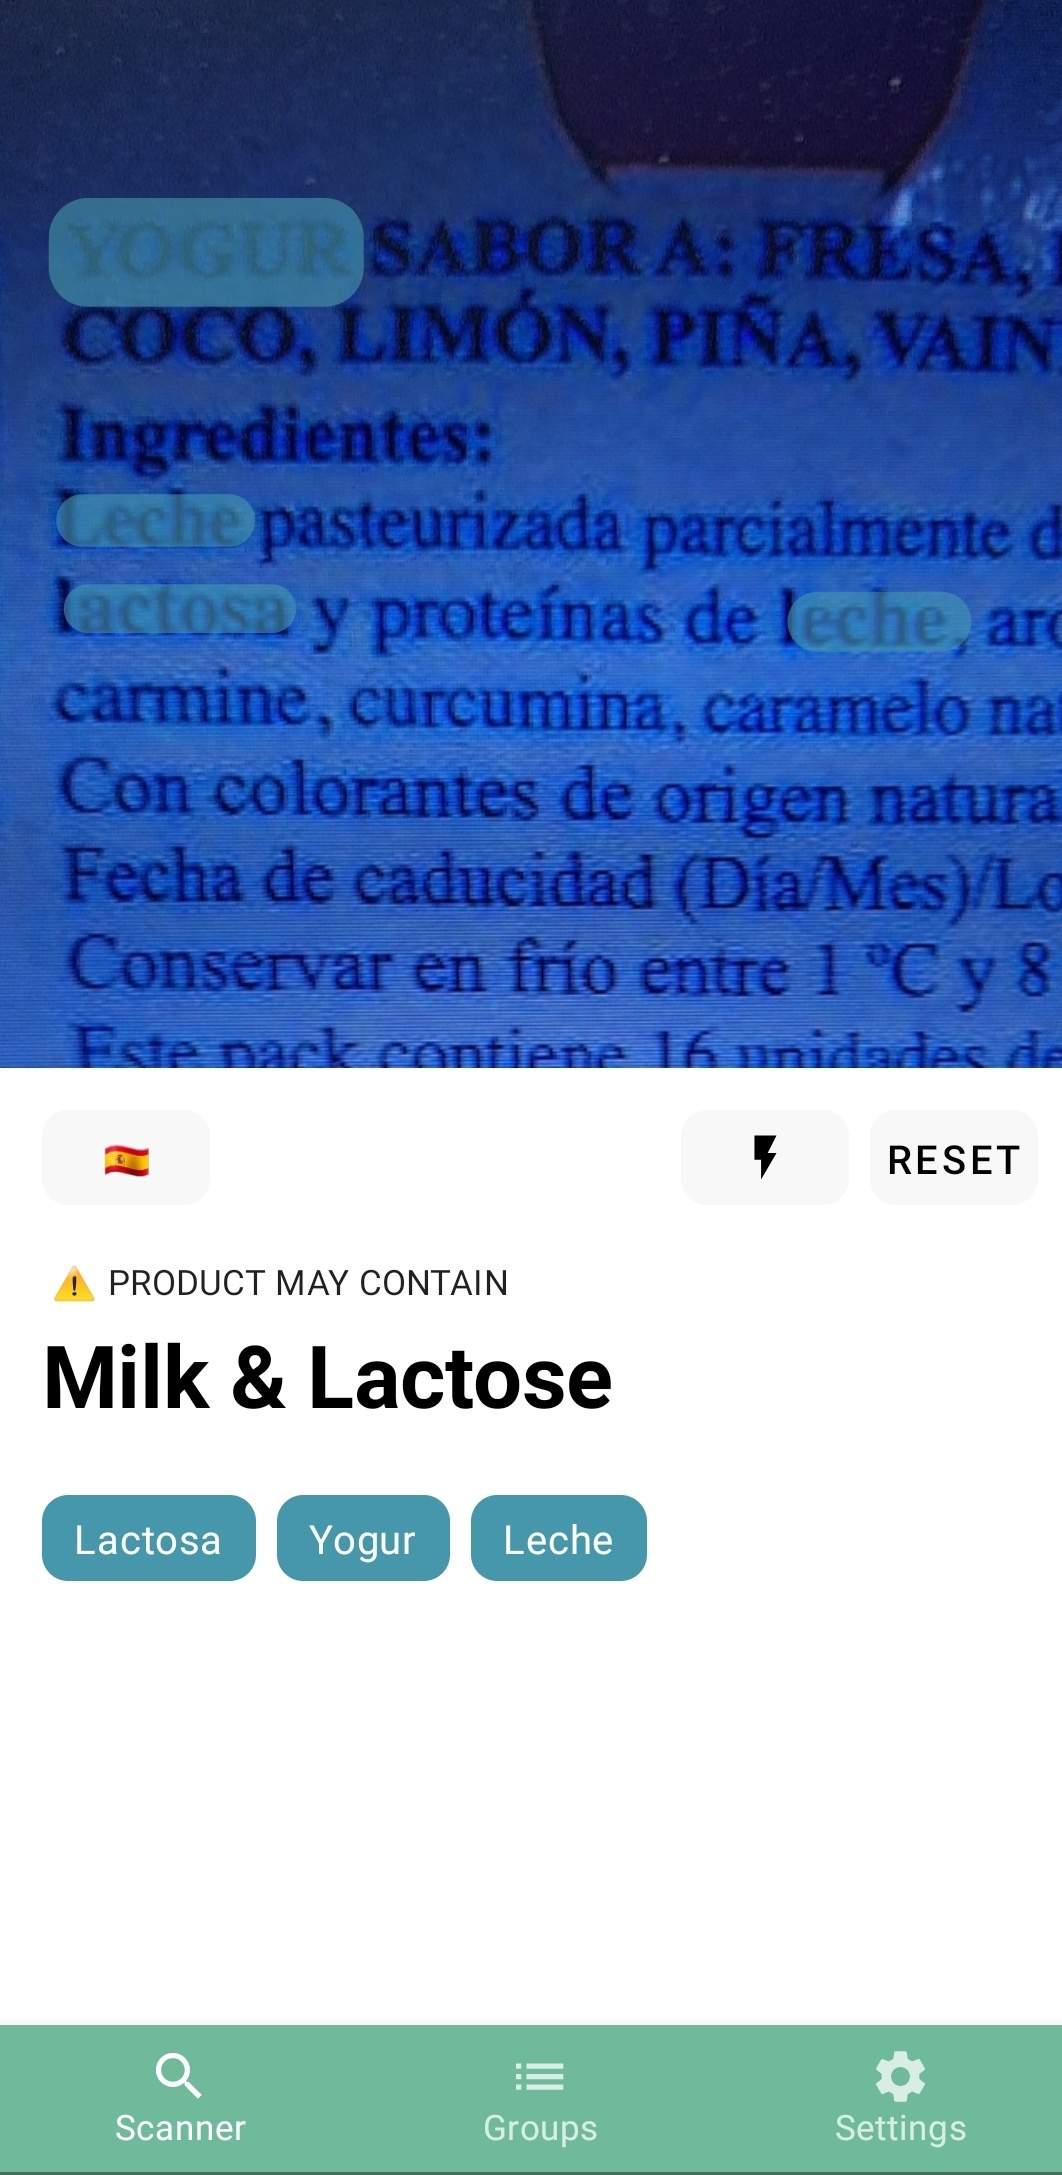
\includegraphics[width=0.9\linewidth]{Figures/soosee-1.jpg}
        \caption{}
        \label{fig:soosee-1}
    \end{subfigure}
    \begin{subfigure}{0.3\textwidth}
        \centering
        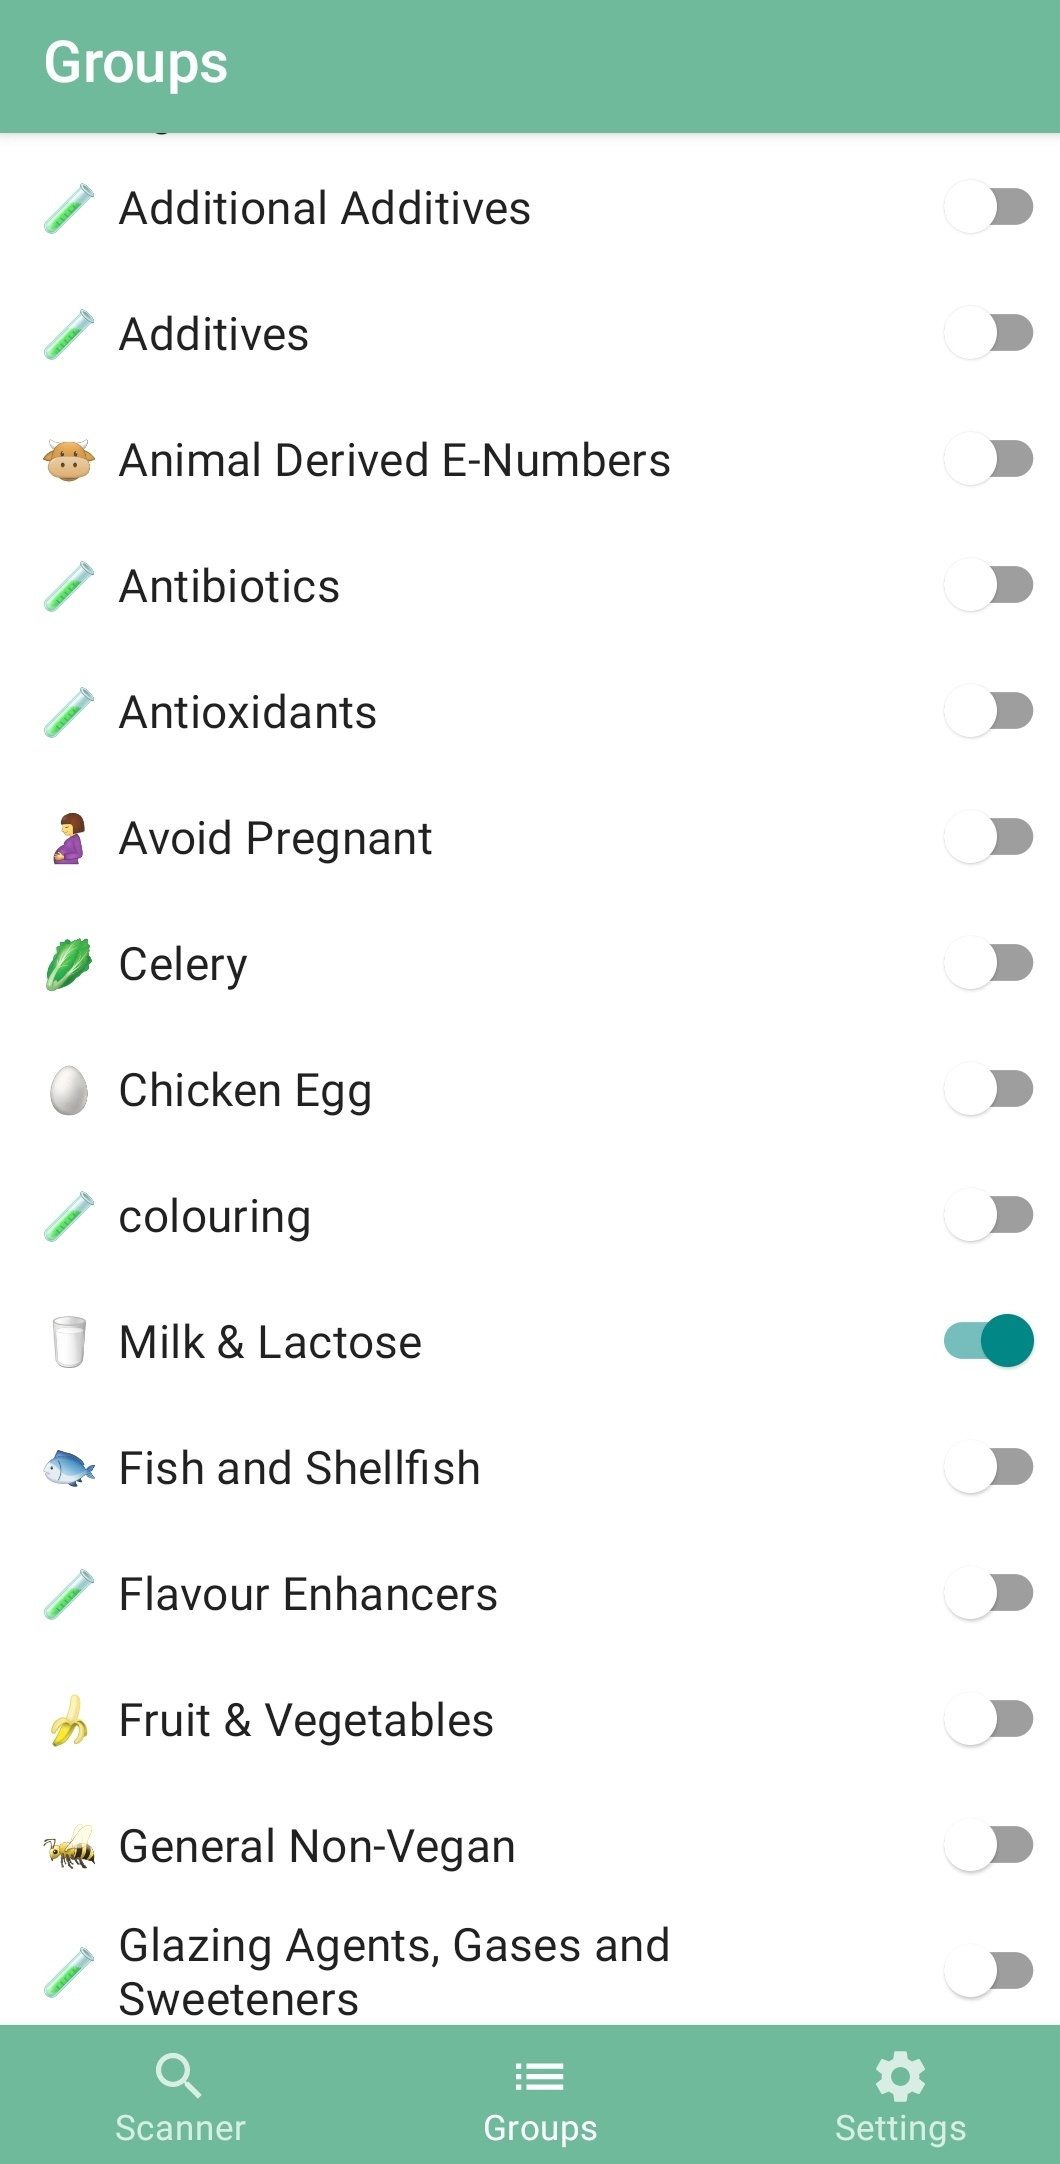
\includegraphics[width=0.9\linewidth]{Figures/soosee-2.jpg}
        \caption{}
        \label{fig:soosee-2}
    \end{subfigure}
    \begin{subfigure}{0.3\textwidth}
        \centering
        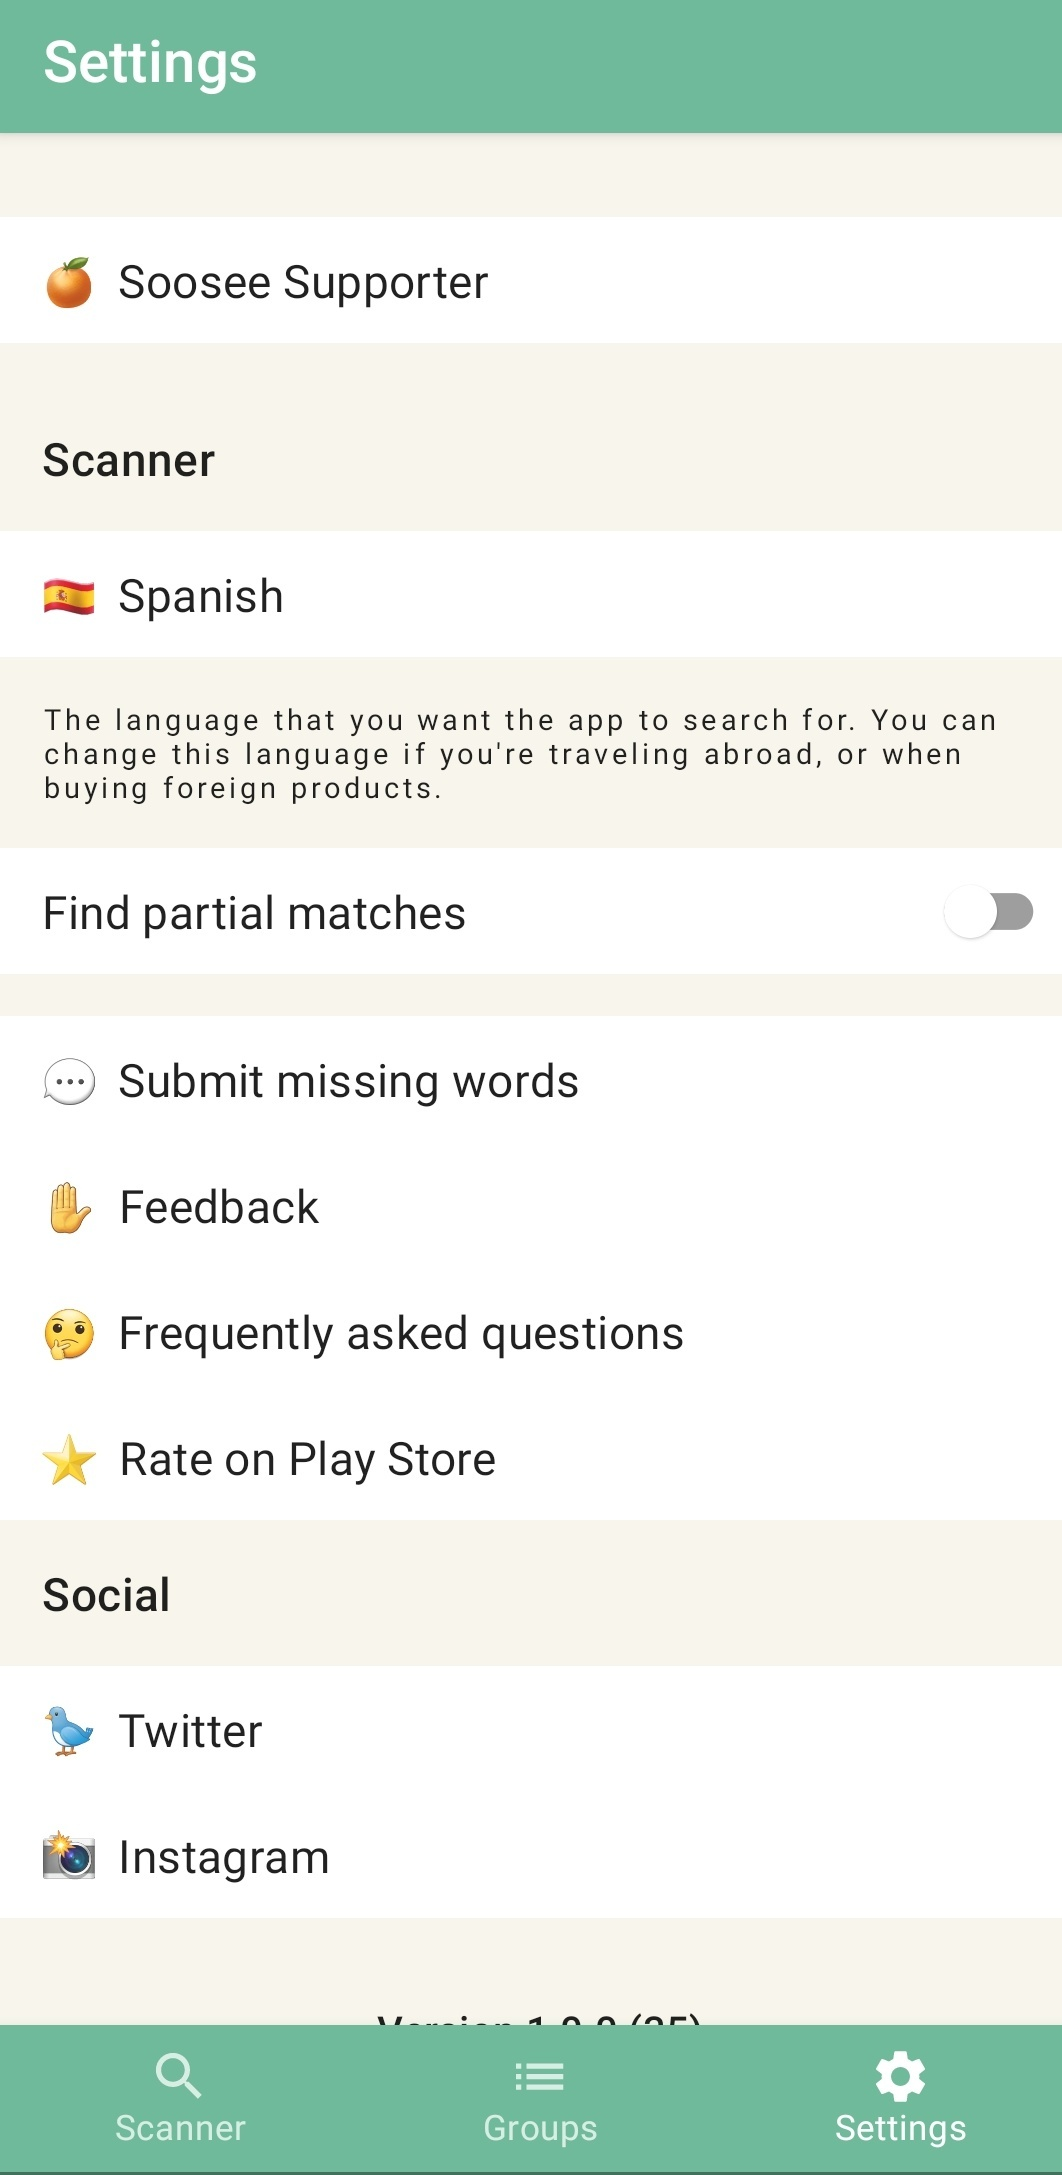
\includegraphics[width=0.9\linewidth]{Figures/soosee-3.jpg}
        \caption{}
        \label{fig:soosee-3}
    \end{subfigure}
    \caption{Soosee app screenshots}
    \label{fig:soosee-screenshot}
\end{figure}

\section{Feature comparison}

In Table \ref{tab:comparison}, we can see a summary of the comparison made on the previous sections. This table aims to include and compare those features that are more desirable for a user with food intolerances that primarily needs Korean support, English output and alerts when specific ingredients are found.

Under these assumptions, we can conclude that our app is the best choice for a user with these needs, supporting up to 6 features out of the 8 that were studied.
 
\begin{table}[h]
\centering
\begin{tabular}{@{}lccccc@{}}
\toprule
\textbf{}               & \textbf{Kamis et al.} & \textbf{Jacky et al.} & \textbf{Yuka} & \textbf{Soosee} & \textbf{Ours} \\ \midrule
Scanning of Korean text & -                     & \checkmark            & -             & -               & \checkmark    \\
Translation             & -                     & -                     & -             & -               & \checkmark    \\
Search history          & -                     & -                     & \checkmark    & -               & \checkmark    \\
Custom ingredients      & -                     & -                     & -             & \checkmark      & \checkmark    \\
Ingredient alerts       & \checkmark            & -                     & -             & \checkmark      & \checkmark    \\
Cross-language          & -                     & \checkmark            & \checkmark    & \checkmark      & \checkmark    \\
Barcode scanning        & -                     & -                     & \checkmark    & -               & -             \\
Real-time results       & -                     & -                     & -             & \checkmark      & -             \\ \bottomrule
\end{tabular}
\caption{%
    Feature comparison across all alternatives
}
\label{tab:comparison}
\end{table}